\chapter{Numerical results}\label{ch:numerical_results}
In this section we present the results of the numerical experiments, together with the results from the data-driven methods, including neural networks and Fourier neural operators.
In \autoref{ch:numerical_results} we present the results from the finite volume method (FVM), where we have implemented the method for solving the shallow water equations in 1D  and 2D and tested it on several problems.
We also address the scalability issues of the FVM.
In \autoref{ch:data-driven-results} we present the results from the data-driven methods, where we have implemented neural networks and Fourier neural operators to solve the shallow water equations in 1D.
We compare the results from the data-driven methods with the results from the FVM, and discuss the advantages and disadvantages of the different methods.
We expand and in \autoref{sec:data-driven-results-2D} we present the results from the data-driven methods for solving the shallow water equations in 2D.

In this chapter we present the results of the numerical experiments, where we have implemented the finite volume method for solving the shallow water equations in 1D and tested it on several problems.
\footnote{Code and small animations can be found at github, visit \url{https://github.com/MelissaJessen/Shallow-Water-Equations}.}
A key focus is to validate the implementation, as it will generate data for the data-driven methods, including neural networks and Fourier neural operators.
To test the implementation, we have solved the 1D dam break problem, and the five test cases from Toro (2001)~\cite{Toro2001-Shock}.
These problems are all discontinuous in either the water height $h$ or the fluid velocity $u$.
The idea is, that if the numerical solution can capture the discontinuities, it should be well-suited to handle smoother solutions as well.
Finally, we have tested the implementation on the 2D idealised circular dam break problem, which is also from Toro (2024)~\cite{Toro2024}.
The results from the 2D problem are compared to the results from the book to validate the implementation.
Lastly, we have tested the scalability of the FVM to solve the 2D SWE, by running the 2D problem with a Gaussian initial condition for different values of $N$, i.e., the number of cells in each direction.

The used computer for running simulations is a Windows 11 computer with an Intel Core i7 CPU and 16 GB of RAM.
All code and data can be found at the Github repository~\cite{Github_SWE}.


\section{The 1D Dam Break Problem}
First we solve the 1D dam break problem, with the following initial conditions:
\begin{align*}
    h(x,0) &= \begin{cases}
        h_L, & \text{if } x < x_0, \\
        h_R, & \text{if } x > x_0,
    \end{cases} 
\end{align*}
where $x \in [0 \text{ m}, 50 \text{ m}]$, $h_L = 3.5$ m, $h_R = 1.25$ m and $x_0 = 20$ m.
Since it is a dam break problem the initial fluid velocity is zero, i.e., $u(x,0) = 0$ m/s.
We solve the problem starting at $t=0$ s and ending at $t=2.5$ s.
The numerical solution to the 1D Dam Break Problem using the FVM, together with the true solution, provided from the course~\cite{phd_corse_2009}, can be seen in \autoref{fig:1D_dam_break}.
\begin{figure}[H]
    \centering
    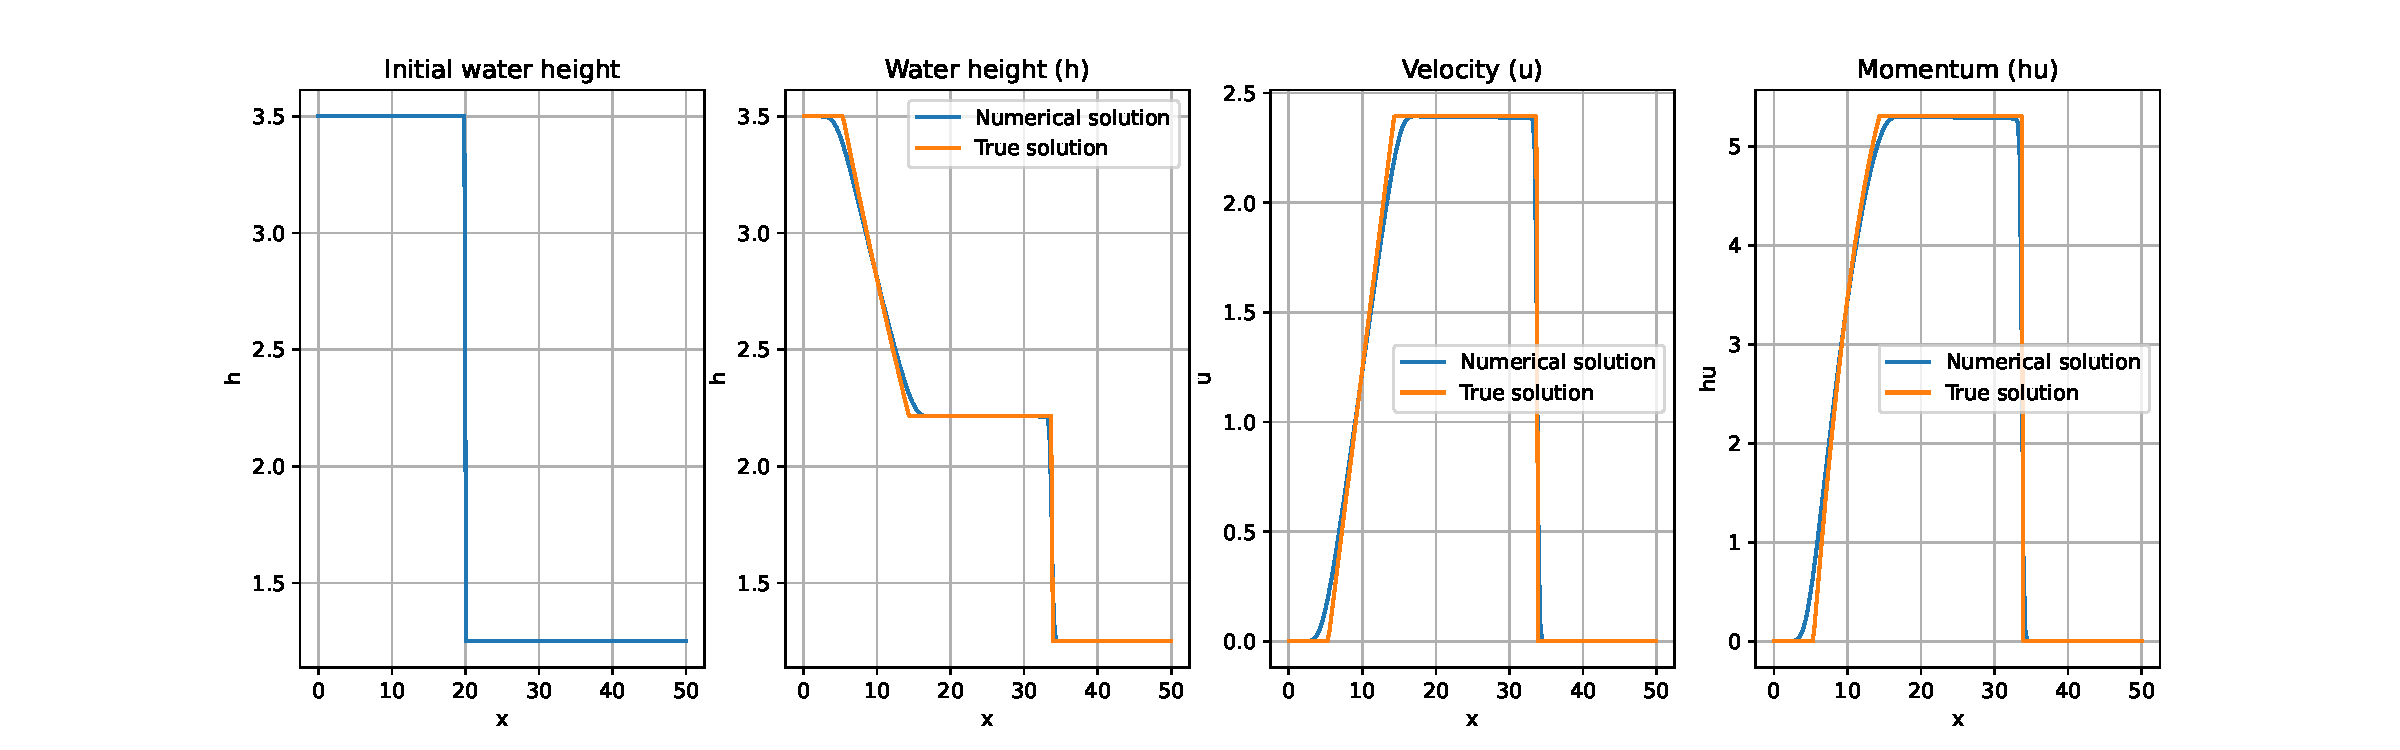
\includegraphics[width=0.99\textwidth]{C:/Users/Matteo/Shallow-Water-Equations/plots/sol_1D_val.pdf}
    \caption{The initial water height $h$ at $t=0$ s, together with the water height, the fluid velocity $u$ and the momentum $hu$ at $t=2.5$ s.}\label{fig:1D_dam_break}
\end{figure}
From Figure~\ref{fig:1D_dam_break} we see that the numerical solution aligns well with the true solution, and successfully captures the discontinuity.


\section{Toro test cases}
We have tested the method on the five test cases for Riemann problems from Toro (2001)~\cite{Toro2001-Shock}.
The initial conditions for the five test cases are given in \autoref{tab:toro_test_cases}.
\begin{table}[H]
    \centering
    \begin{tabular}{c|c|c|c|c|c|c}
        \hline
        \textbf{Test case} & \textbf{$h_L$} [m] & \textbf{$u_L$} [m/s] & \textbf{$h_R$} [m] & \textbf{$u_R$} [m/s] & \textbf{$x_0$} [m] & \textbf{$t_{end}$} [s] \\
        \hline\hline
        1 & 1.0 & 2.5 & 0.1 & 0.0 & 10.0 & 7.0 \\
        2 & 1.0 & -5.0 & 1.0 & 5.0 & 25.0 & 2.5 \\
        3 & 1.0 & 0.0 & 0.0 & 0.0 & 20.0 & 4.0 \\
        4 & 0.0 & 0.0 & 1.0 & 0.0 & 30.0 & 4.0 \\
        5 & 0.1 & -3.0 & 0.1 & 3.0 & 25.0 & 5.0 \\
        \hline
    \end{tabular}
    \caption{Initial conditions for the five test cases.}\label{tab:toro_test_cases}
\end{table}
The domain is $x \in [0 \text{ m}, 50 \text{ m}]$ for all test cases.
The Riemann problems are chosen to test the method on different types of waves, such as shock waves and rarefaction waves.
To solve the test cases we have used the following fluxes:
\begin{enumerate}
    \item Godunov method with exact Riemann solver,
    \item Lax-Friedrich flux,
    \item Lax-Wendroff flux,
    \item FORCE flux,
    \item HLL flux,
\end{enumerate}

\subsection*{Test case 1}
%\addcontentsline{toc}{subsection}{Test case 1}
The initial conditions for test case 1 are given in \autoref{fig:toro_test1_initial} and the final solutions after $t=7.0$ seconds are given in \autoref{fig:toro_test1_final}.
In test case 1, we observe a right shock wave and a left rarefaction wave.
\begin{figure}[H]
    \centering
    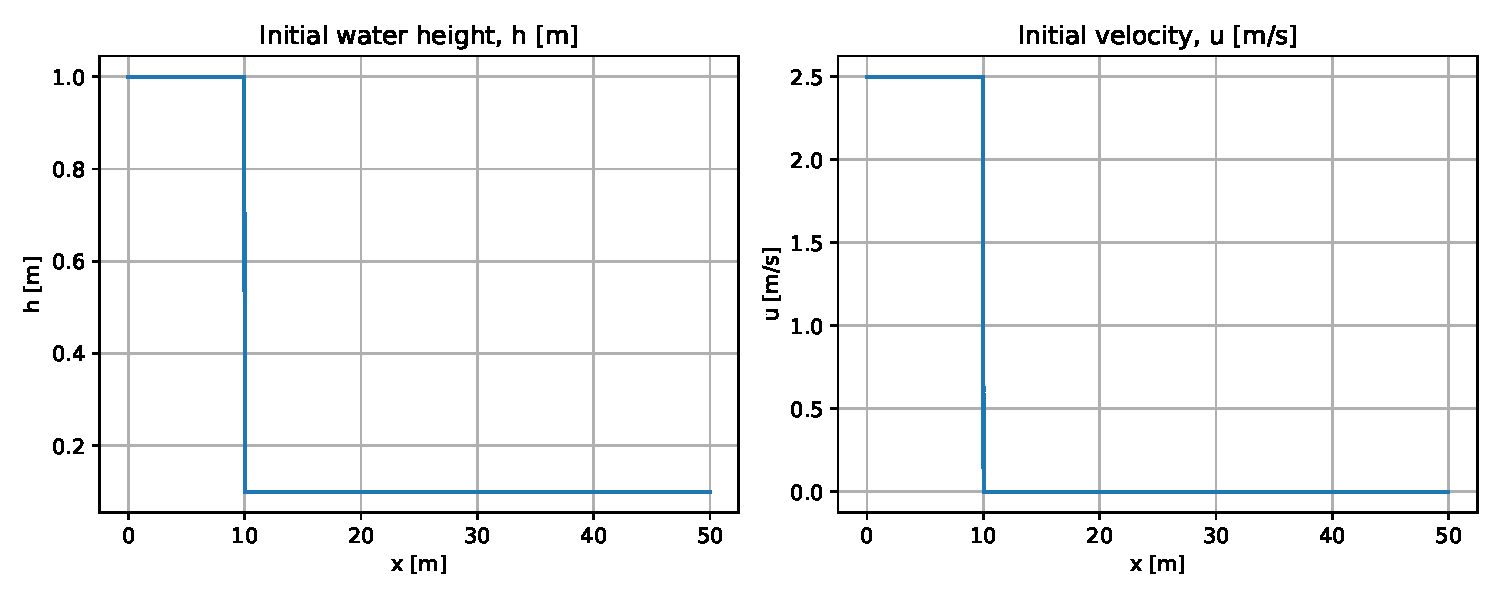
\includegraphics[width=0.9\textwidth]{C:/Users/Matteo/Shallow-Water-Equations/plots/toro_test1_initial.pdf}
    \caption{Initial conditions for the test case.}\label{fig:toro_test1_initial}
\end{figure}

\begin{figure}[H]
    \centering
    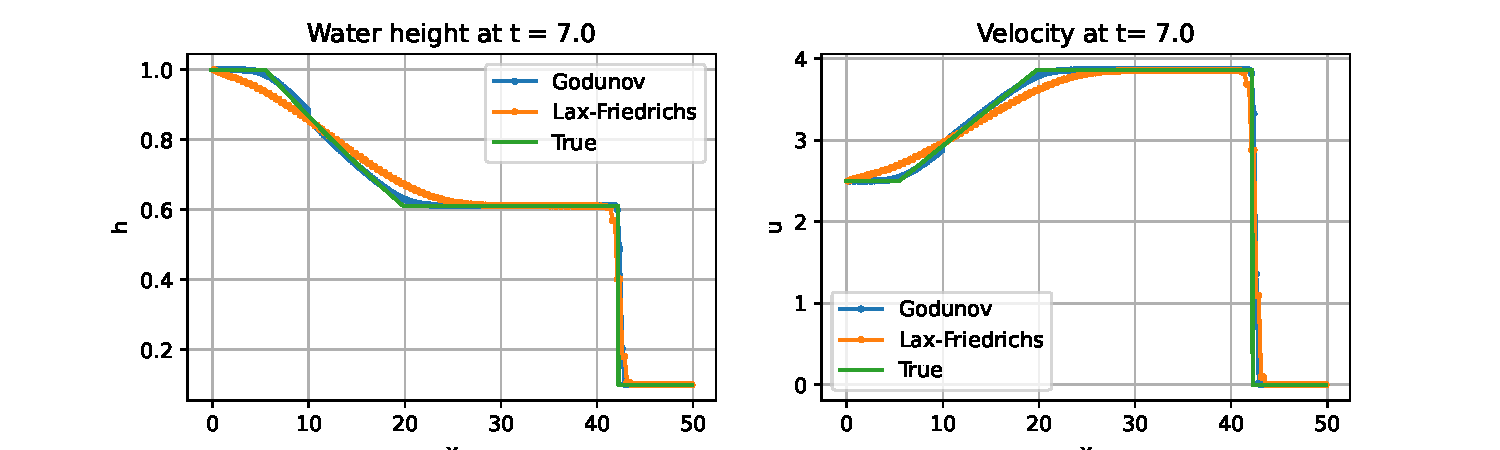
\includegraphics[width=0.9\textwidth]{C:/Users/Matteo/Shallow-Water-Equations/plots/toro_test1_final.pdf}
    \caption{Final solution for the test case.}\label{fig:toro_test1_final}
\end{figure}
For this test case all the fluxes work well, but there are minor differences in the solution, which can be seen in \autoref{fig:toro_test1_final}.
We also see that Lax-Wendroff flux has some oscillations in the solution, which is not present in the other fluxes.

\subsection*{Test case 2}
%\addcontentsline{toc}{subsection}{Test case 2}
The initial conditions for test case 2 are illustrated in \autoref{fig:toro_test2_initial}.
\begin{figure}[H]
    \centering
    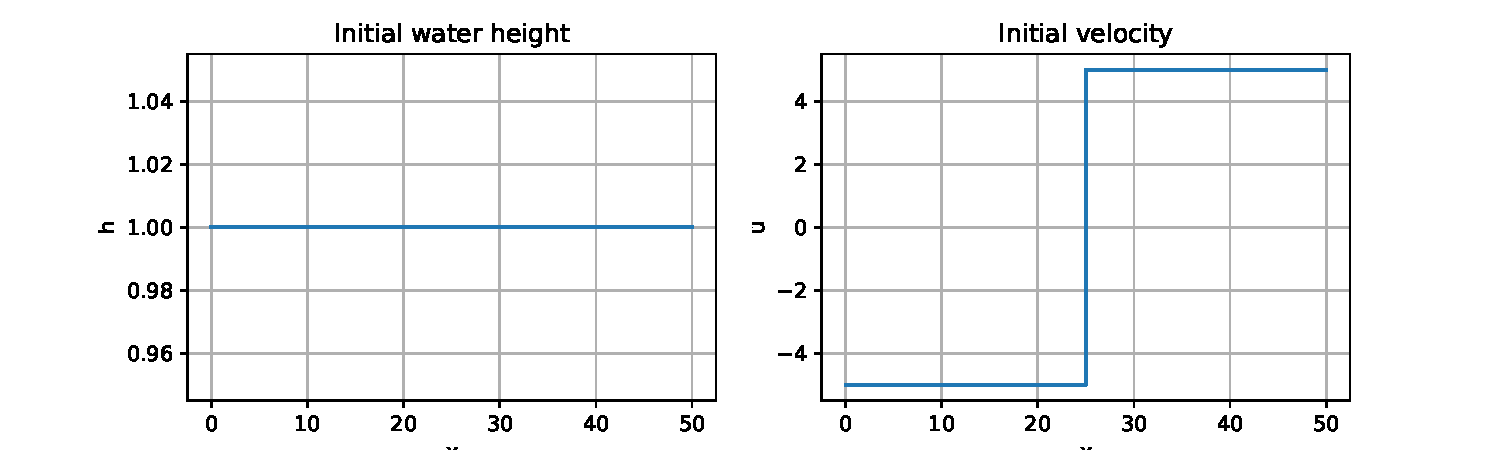
\includegraphics[width=0.9\textwidth]{C:/Users/Matteo/Shallow-Water-Equations/plots/toro_test2_initial.pdf}
    \caption{Initial conditions for the test case.}\label{fig:toro_test2_initial}
\end{figure}
In test case 2 we have two rarefaction waves, one on the left side and one on the right side.
As they are travelling in opposite directions (away from each other), there will be created a nearly dry bed in the middle of the domain.
Many methods have difficulties with this test case as they may compute a negative water height.
For these experiments we were able to get close to the true solution, using Lax-Friedrich flux, FORCE flux and HLL flux.
The final solutions after $t=2.5$ seconds are illustrated in \autoref{fig:toro_test2_final}.
\begin{figure}[H]
    \centering
    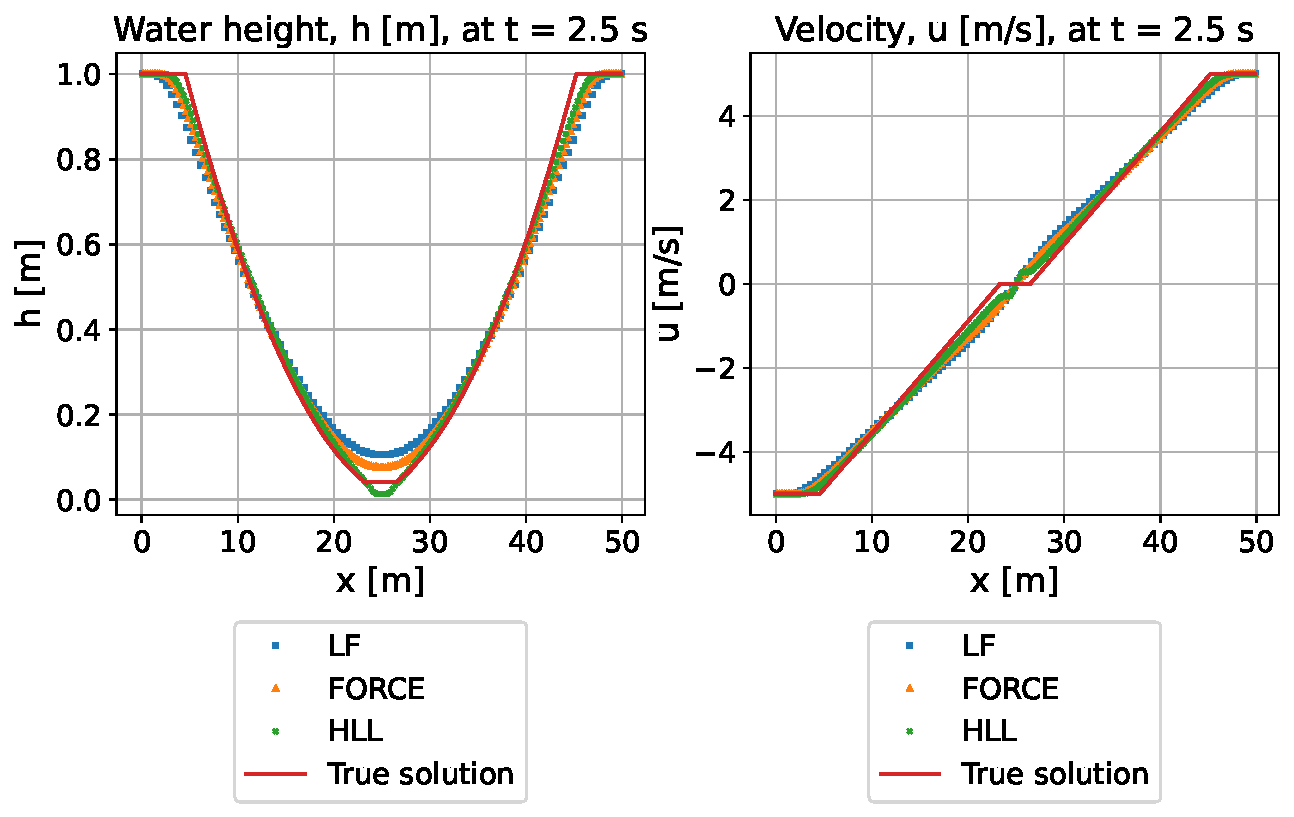
\includegraphics[width=0.9\textwidth]{C:/Users/Matteo/Shallow-Water-Equations/plots/toro_test2_final.pdf}
    \caption{Final solution for the test case.}\label{fig:toro_test2_final}
\end{figure}
For the fluxes, Godunov method with exact Riemann solver, and Lax-Wendroff, it was not possible to get an acceptable solution.

\subsection*{Test case 3}
%\addcontentsline{toc}{subsection}{Test case 3}
The initial conditions for test case 3 are given in \autoref{fig:toro_test3_initial}, and the final solutions after $t=4.0$ seconds are given in \autoref{fig:toro_test3_final}.
\begin{figure}[H]
    \centering
    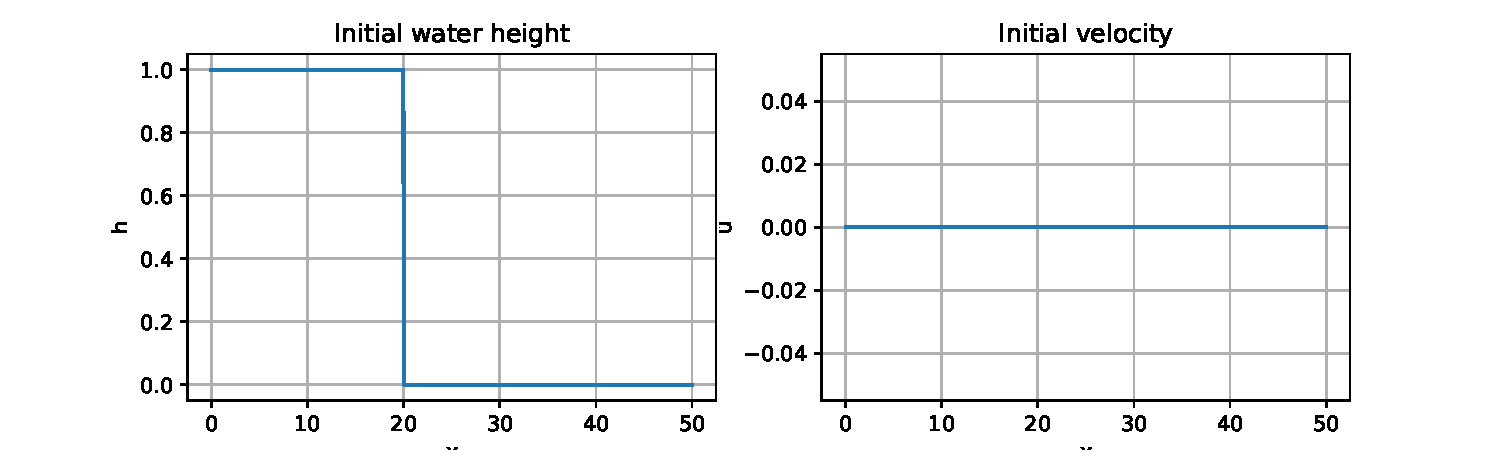
\includegraphics[width=0.9\textwidth]{C:/Users/Matteo/Shallow-Water-Equations/plots/toro_test3_initial.pdf}
    \caption{Initial conditions for the test case.}\label{fig:toro_test3_initial}
\end{figure}

\begin{figure}[H]
    \centering
    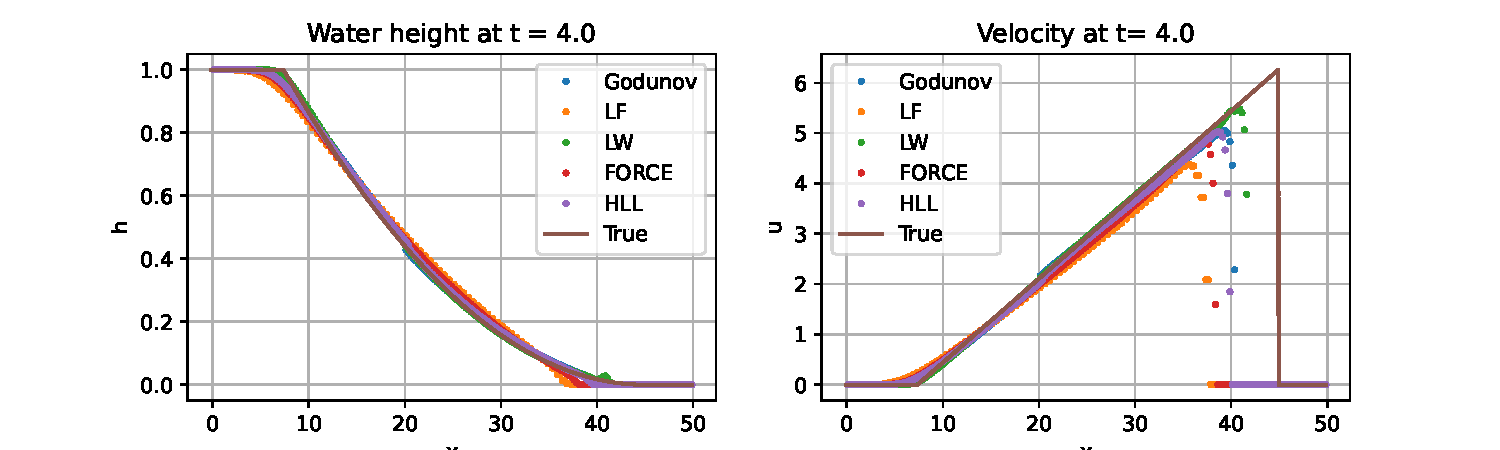
\includegraphics[width=0.9\textwidth]{C:/Users/Matteo/Shallow-Water-Equations/plots/toro_test3_final.pdf}
    \caption{Final solution for the test case.}\label{fig:toro_test3_final}
\end{figure}
To solve case 3, with the FVM we must add a small amount to $h_R$, since the code does not handle $h_R = 0$ well.
We set $h_R = 0.00005$ to solve it numerically, but the true solution is for $h_R = 0$.
By running experiments with different values of $h_R$, we see that the solution converges to the true solution as $h_R$ approaches 0.
The solution consists of a left rarefaction wave.
From \autoref{fig:toro_test3_final} we see that when it comes to predicting the velocity, there are some differences in how the different fluxes perform.

\subsection*{Test case 4}
%\addcontentsline{toc}{subsection}{Test case 4}
The initial conditions for test case 4 are given in \autoref{fig:toro_test4_initial}, and the final solutions after $t=4.0$ seconds are given in \autoref{fig:toro_test4_final}.
\begin{figure}[H]
    \centering
    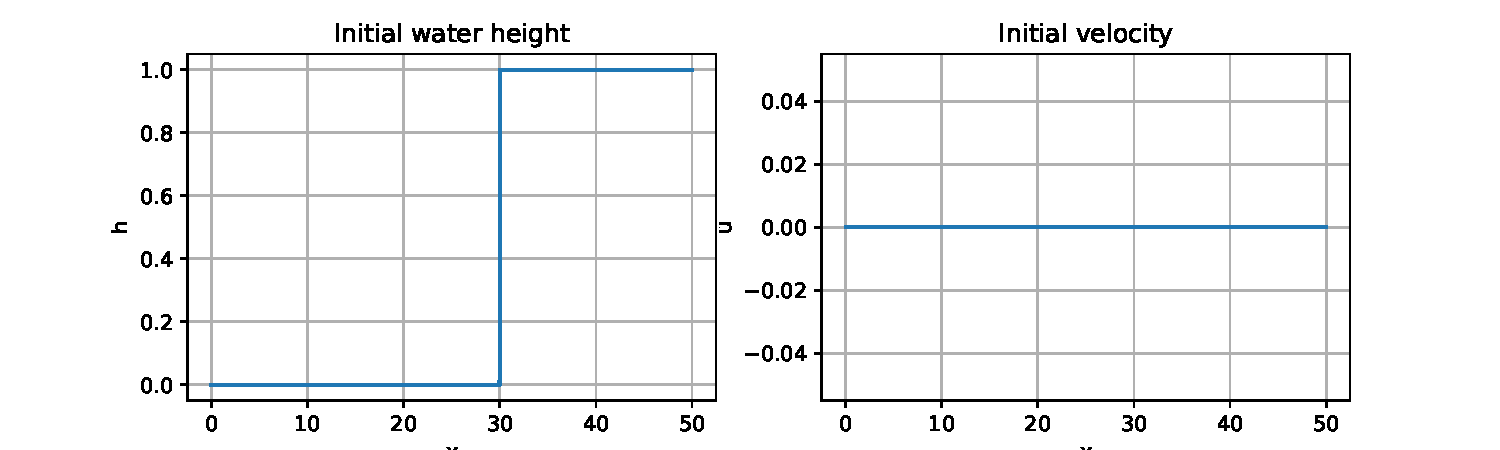
\includegraphics[width=0.9\textwidth]{C:/Users/Matteo/Shallow-Water-Equations/plots/toro_test4_initial.pdf}
    \caption{Initial conditions for the test case.}\label{fig:toro_test4_initial}
\end{figure}

\begin{figure}[H]
    \centering
    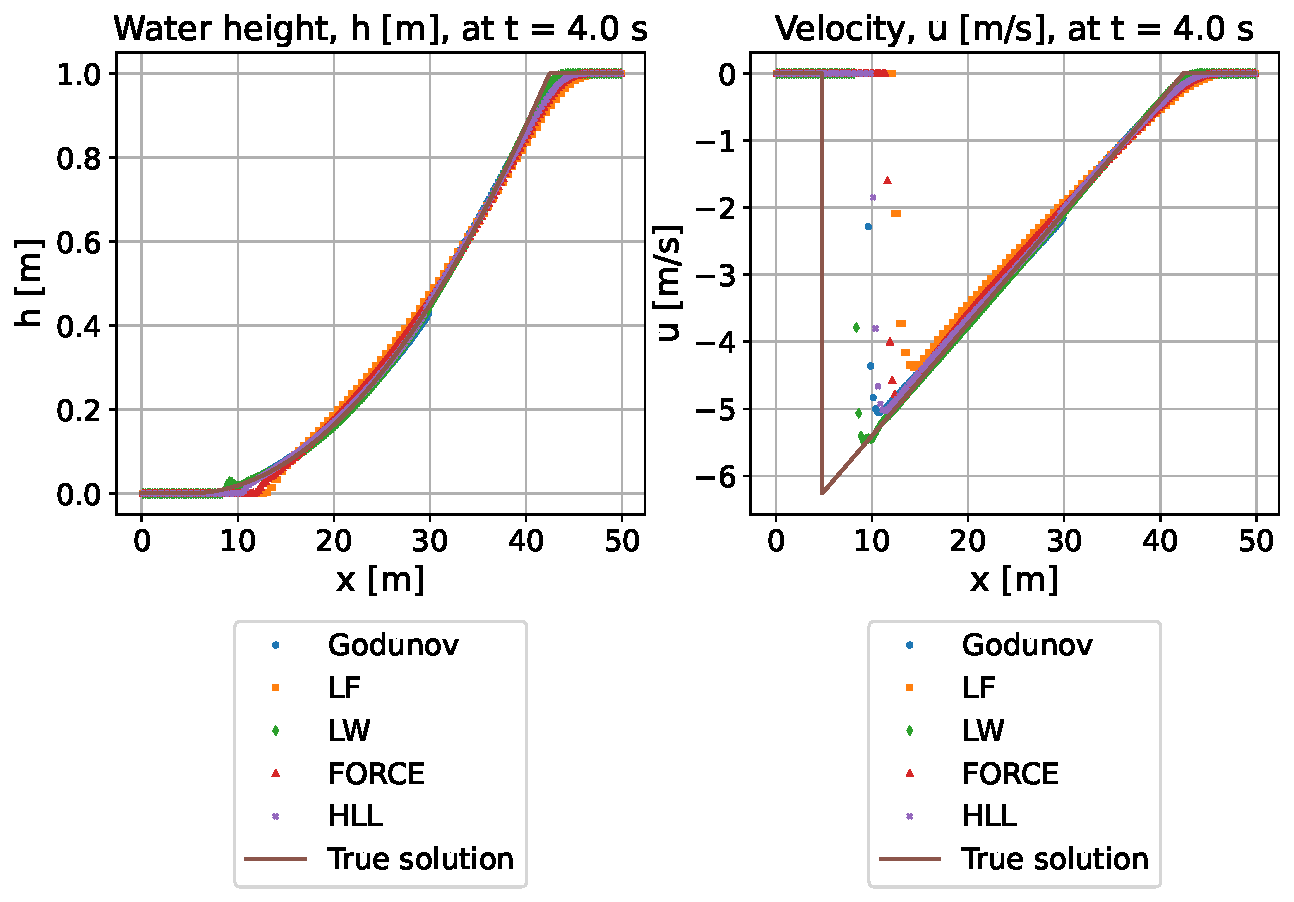
\includegraphics[width=0.9\textwidth]{C:/Users/Matteo/Shallow-Water-Equations/plots/toro_test4_final.pdf}
    \caption{Final solution for the test case.}\label{fig:toro_test4_final}
\end{figure}
In case 4 we face the same challenges as in case 3.
We set $h_L = 0.00005$, and the solution converges to the true solution as $h_L$ approaches 0.
This test case is symmetric to test case 3, and the solution consists of a right rarefaction wave.
The case is included to test if the results are as expected.
As in test case 4, we observe differences in the fluxes performance.

\subsection*{Test case 5}
%\addcontentsline{toc}{subsection}{Test case 5}
The initial conditions for test case 5 are given in \autoref{fig:toro_test5_initial}, and the final solutions after $t=5.0$ seconds are given in \autoref{fig:toro_test5_final}.
\begin{figure}[H]
    \centering
    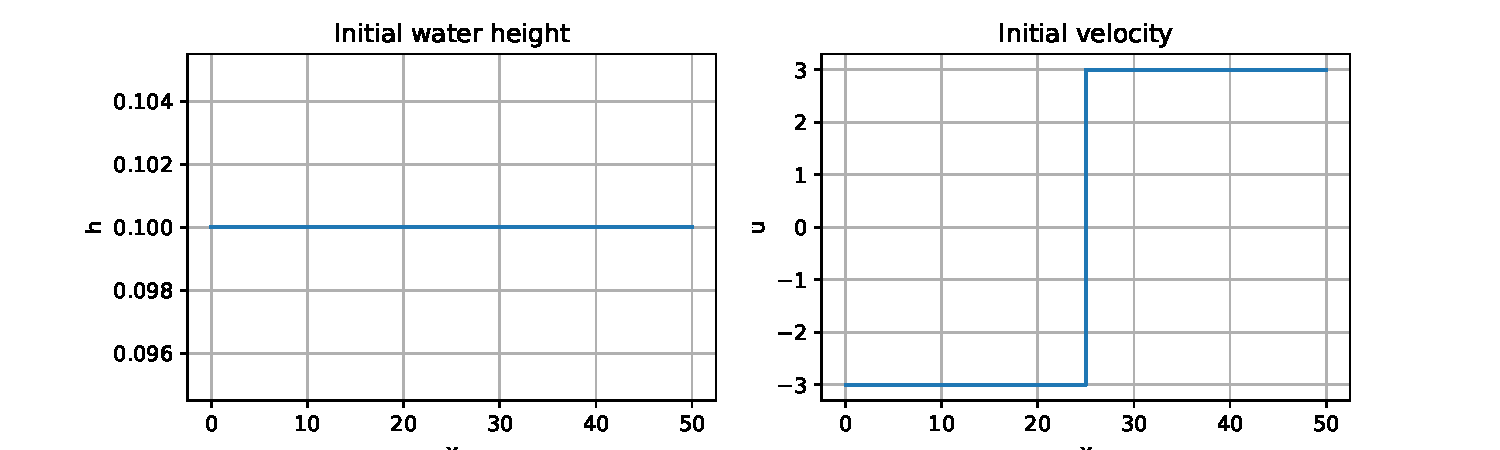
\includegraphics[width=0.9\textwidth]{C:/Users/Matteo/Shallow-Water-Equations/plots/toro_test5_initial.pdf}
    \caption{Initial conditions for the test case.}\label{fig:toro_test5_initial}
\end{figure}

\begin{figure}[H]
    \centering
    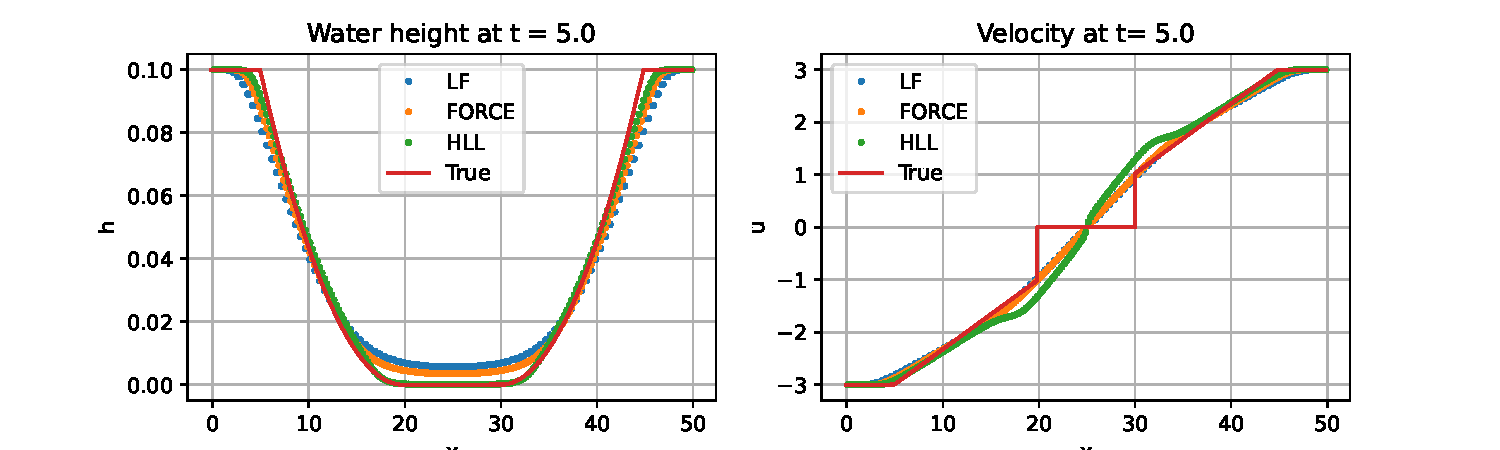
\includegraphics[width=0.9\textwidth]{C:/Users/Matteo/Shallow-Water-Equations/plots/toro_test5_final.pdf}
    \caption{Final solution for the test case.}\label{fig:toro_test5_final}
\end{figure}
From~\autoref{fig:toro_test5_final} we see that the numerical solutions for the velocity $v$ at $t=5.0$ are smooth, where the true solution is discontinuous. 
In this test case there are also challenges with some of the fluxes due to the generation of a dry-bed region.
The fluxes that are not able to solve this case are Godunov method with exact Riemann solver and Lax-Wendroff flux, the same as in test case 2.
The solution consists of two rarefaction waves, one on the left side and one on the right side, and a dry-bed region in the middle.

To get an overview of which fluxes that were able to produce solutions for the test cases, consider~\autoref{tab:toro_fluxes}.
The table shows which fluxes that were able to produce a solution for the test cases.
\begin{table}[H]
    \centering
    \begin{tabular}{c|c|c|c|c|c}
        \hline
        \textbf{Test case} & \textbf{Godunov} & \textbf{LF} & \textbf{LW} & \textbf{FORCE} & \textbf{HLL}   \\
        \hline\hline
        1 & $\checkmark$ & $\checkmark$ & $\checkmark$ & $\checkmark$ & $\checkmark$   \\
        2 & $\times$ & $\checkmark$ & $\times$ & $\checkmark$ & $\checkmark$ \\
        3 & $\checkmark$ & $\checkmark$ & $\checkmark$ & $\checkmark$ & $\checkmark$  \\
        4 & $\checkmark$ & $\checkmark$ & $\checkmark$ & $\checkmark$ & $\checkmark$  \\
        5 & $\times$ & $\checkmark$ & $\times$ & $\checkmark$ & $\checkmark$  \\
        \hline
    \end{tabular}
    \caption{Overview of which fluxes that were able to produce solutions for the test cases.}\label{tab:toro_fluxes}
\end{table}
Note, that as we see in the results, there are still differences in the solutions accuracy between the fluxes that were able to solve the test cases.

\section{2D idealised Circular Dam Break Problem}
We now proceed to the 2D case, focusing on an idealised circular dam break problem over a horizontal bottom.
This problem is also from Toro's book~\cite{Toro2024}.
We assume there is an infinitely thin circular wall at radius $R = 2.5$ m is a square domain of size $40 \text{ m} \times 40 \text{ m}$ with centre at $(x_c,y_c) = (20 \text{ m}, 20 \text{ m})$.
The initial conditions are
\begin{align*}
    h(x,y,0) &= \begin{cases}
        2.5 \text{ m}, & \text{if } \sqrt{ {(x-x_c)}^2 + {(y-y_c)}^2 } \leq R, \\
        0.5 \text{ m}, & \text{otherwise},
    \end{cases} \\
    u(x,y,0) &= 0 \text{ m/s}, \\
    v(x,y,0) &= 0 \text{ m/s}.
\end{align*}
We use a mesh of size $200 \times 200$.
The results after $t=0.0 \text{ s}, 0.4 \text{ s}, 0.7 \text{ s}$ and $1.4$ s are given in \autoref{fig:2D_dam_break_grid}.
\begin{figure}[H]
    \centering
    \begin{subfigure}{0.49\textwidth}
        \centering
        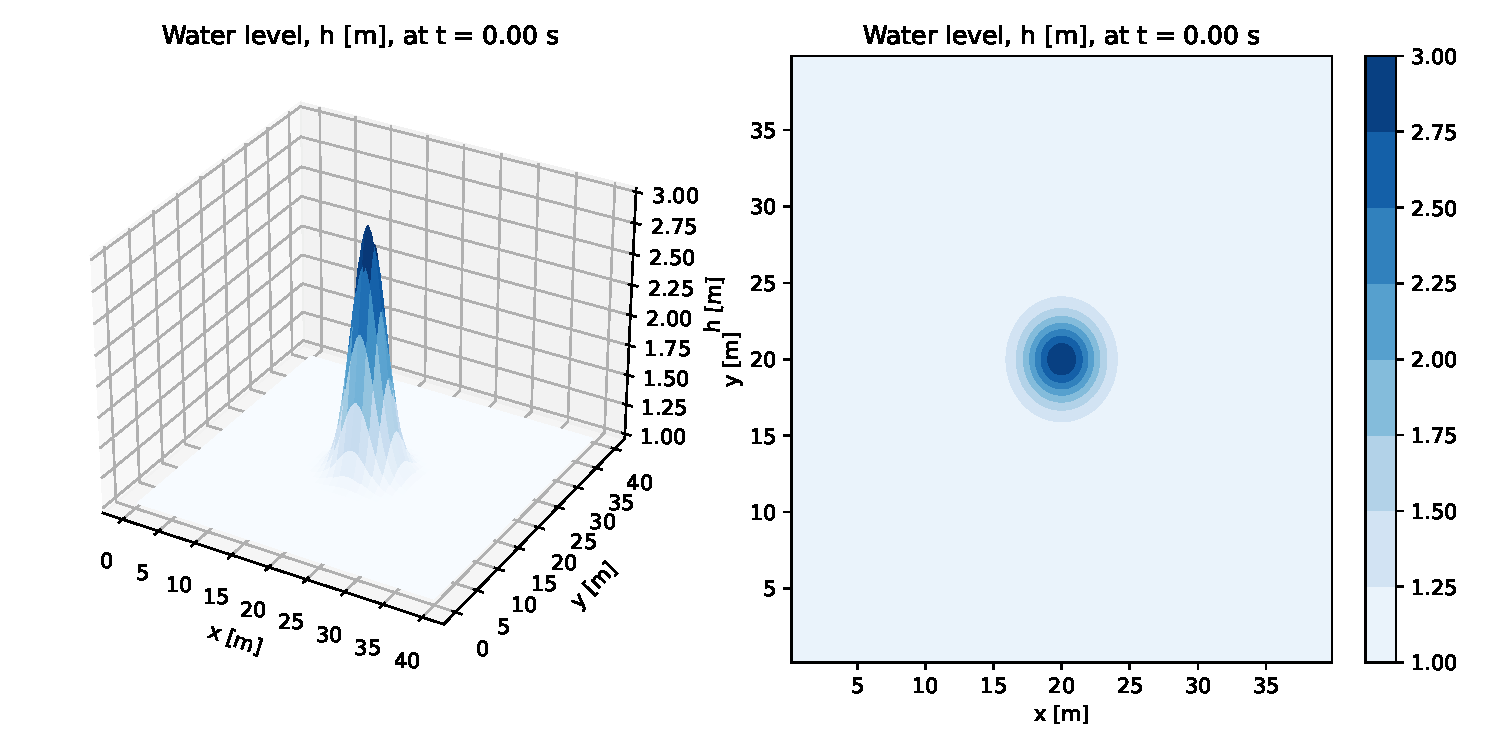
\includegraphics[width=\textwidth]{C:/Users/Matteo/Shallow-Water-Equations/plots/toro2D_t=0.pdf}
        \caption{2D dam break problem after $t=0$ s.}\label{fig:2D_dam_break_t0}
    \end{subfigure}
    \hfill
    \begin{subfigure}{0.49\textwidth}
        \centering
        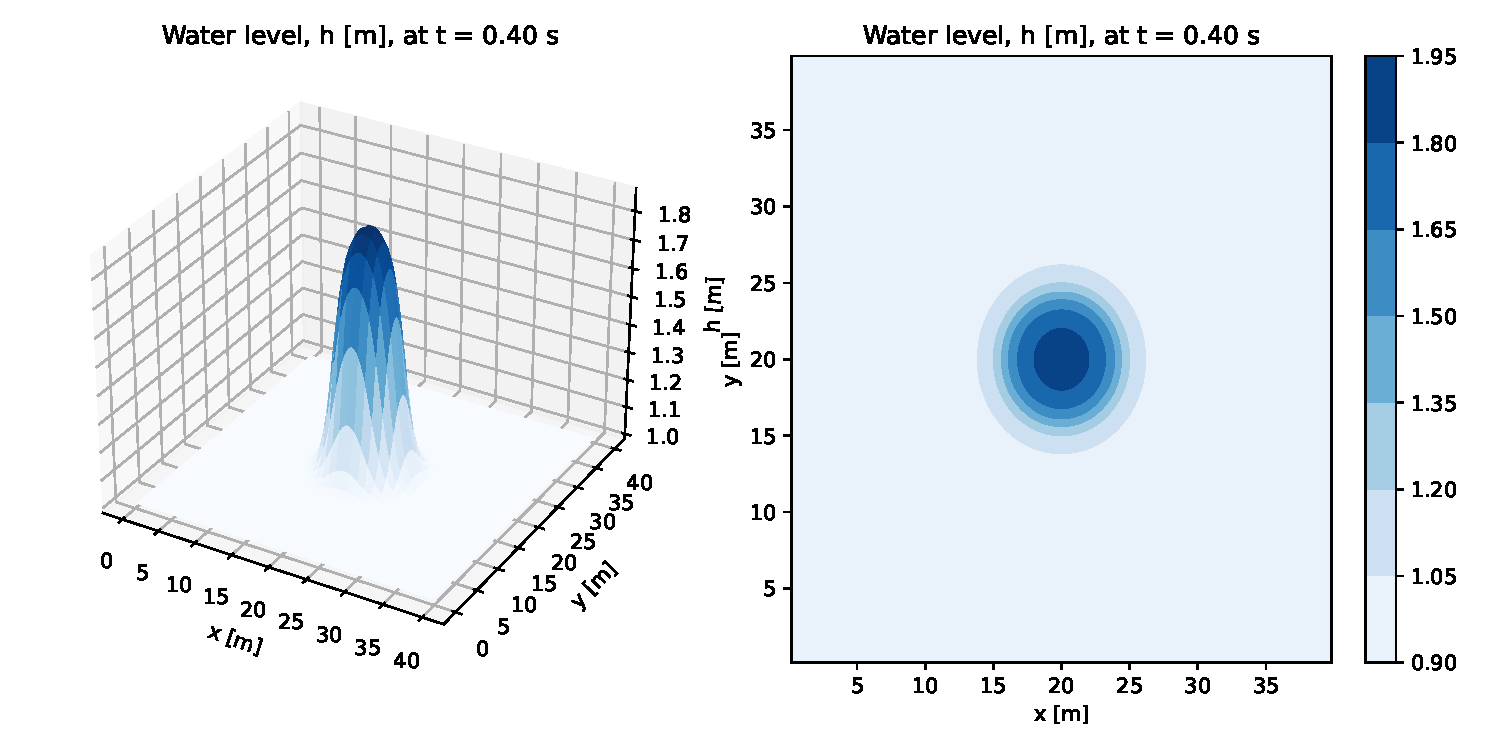
\includegraphics[width=\textwidth]{C:/Users/Matteo/Shallow-Water-Equations/plots/toro2D_t=0.4.pdf}
        \caption{2D dam break problem after $t=0.4$ s.}\label{fig:2D_dam_break_t0.4}
    \end{subfigure}

    \vspace{0.5cm} % Adjusts vertical space between rows

    \begin{subfigure}{0.49\textwidth}
        \centering
        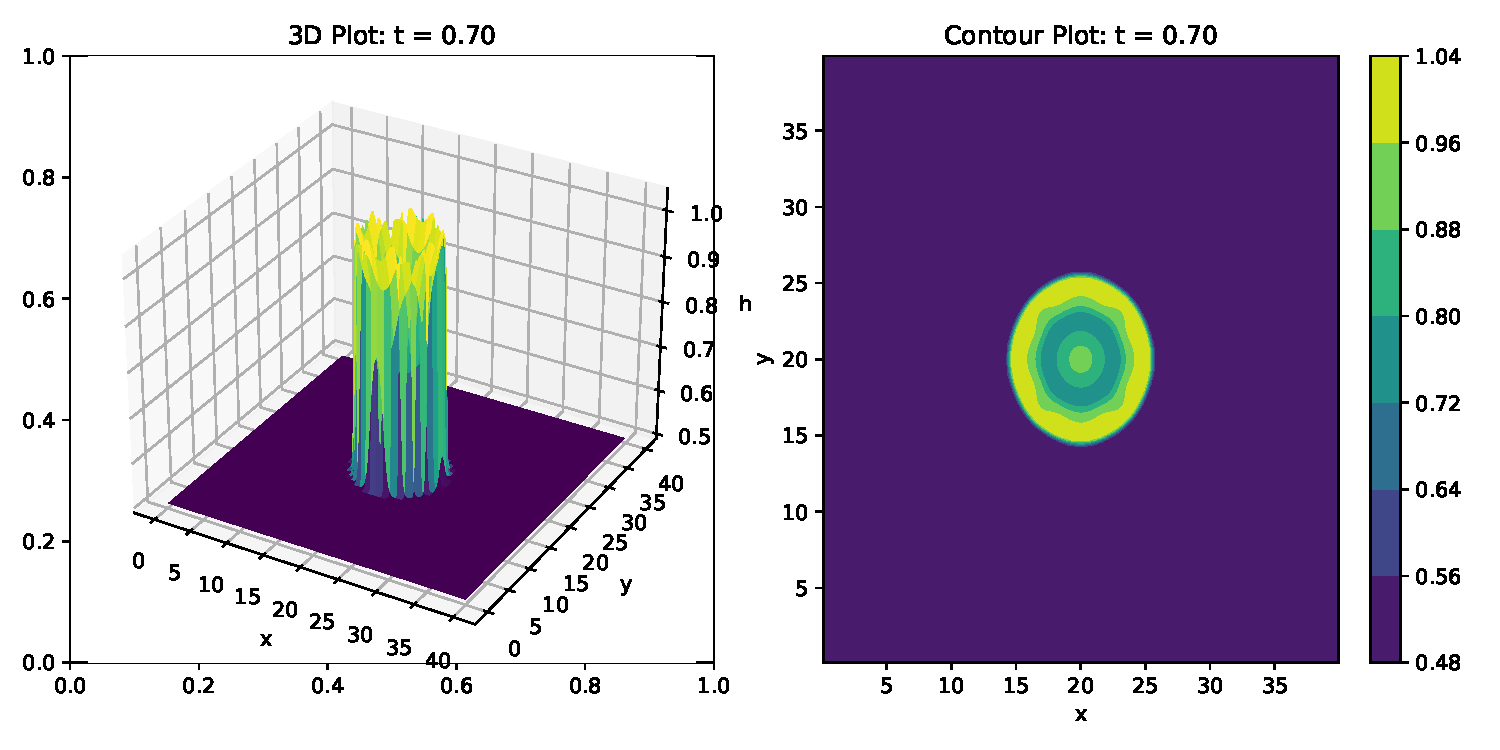
\includegraphics[width=\textwidth]{C:/Users/Matteo/Shallow-Water-Equations/plots/toro2D_t=0.7.pdf}
        \caption{2D dam break problem after $t=0.7$ s.}\label{fig:2D_dam_break_t0.7}
    \end{subfigure}
    \hfill
    \begin{subfigure}{0.49\textwidth}
        \centering
        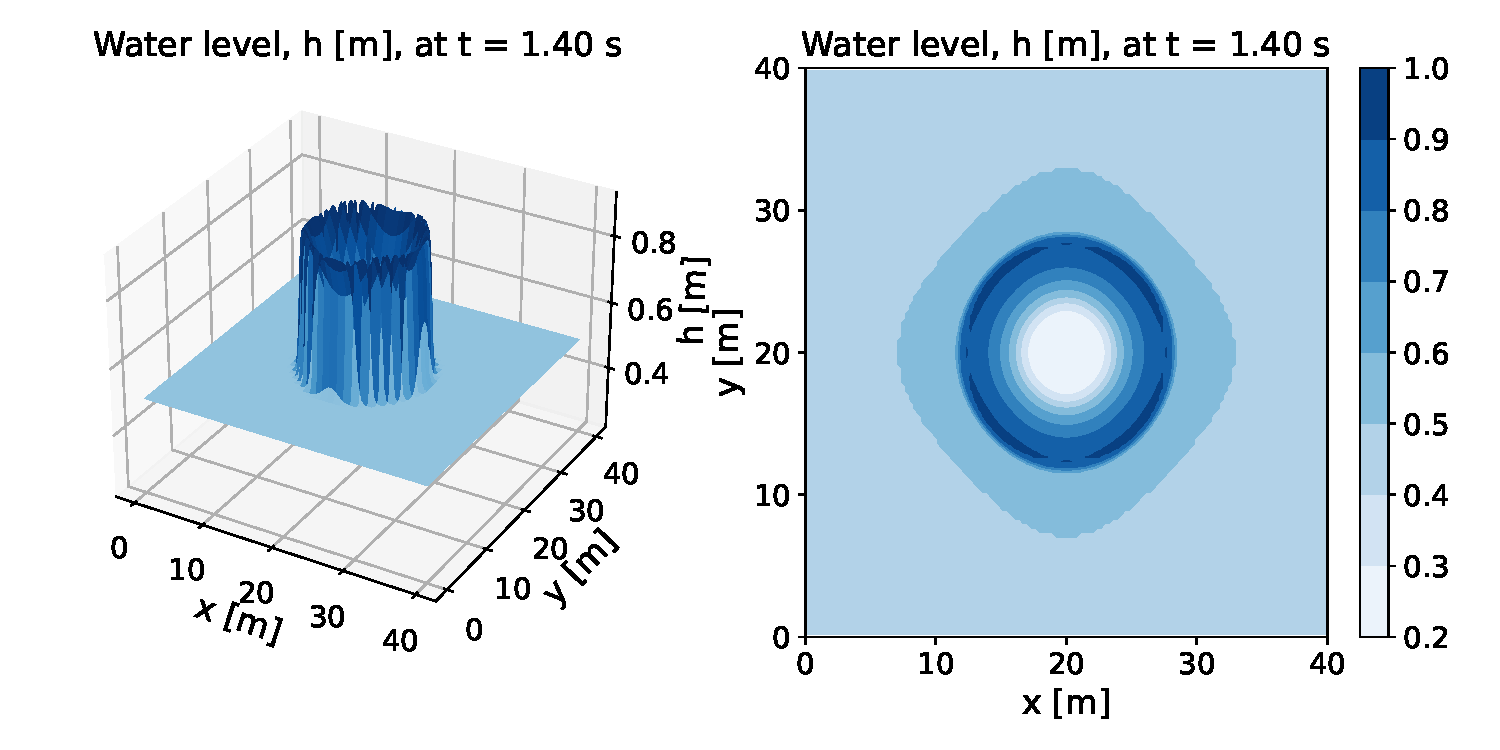
\includegraphics[width=\textwidth]{C:/Users/Matteo/Shallow-Water-Equations/plots/toro2D_t=1.4.pdf}
        \caption{2D dam break problem after $t=1.4$ s.}\label{fig:2D_dam_break_t1.4}
    \end{subfigure}

    \caption{Snapshots of the 2D dam break problem at different times.}\label{fig:2D_dam_break_grid}
\end{figure}

By comparing \autoref{fig:2D_dam_break_grid} with the results from the book by Toro~\cite{Toro2024}, and see that the numerical solution aligns well with the true solution from the book.

\section{Scalability}
To test the scalability of the FVM to solve the 2D SWE, we have run the 2D problem with a Gaussian initial condition, for different values of $N$, i.e., the number of cells in each direction.
Numerical methods are good as they can be more or less as accurate as we want them to be, but the computational cost increases with the number of cells.

\begin{table}[H]
    \centering
    \begin{tabular}{c|ccccc}
        \hline
        $N$ & 16 & 32 & 64 & 128 & 256 \\
        \hline 
        Time ($s$) & 
        \input{C:/Users/Matteo/Shallow-Water-Equations/saved_results/2D_FVM_N=16_time_5.txt} &
        \input{C:/Users/Matteo/Shallow-Water-Equations/saved_results/2D_FVM_N=32_time_5.txt} &
        \input{C:/Users/Matteo/Shallow-Water-Equations/saved_results/2D_FVM_N=64_time_5.txt} &
        \input{C:/Users/Matteo/Shallow-Water-Equations/saved_results/2D_FVM_N=128_time_5.txt} &
        \input{C:/Users/Matteo/Shallow-Water-Equations/saved_results/2D_FVM_N=256_time_5.txt}
        \\
        \hline
    \end{tabular}
    \caption{Running time for the FVM to solve 2D SWE for different values of $N$.}\label{tab:scalability}
\end{table}

The run time dependent of the number of cells $N$ is illustrated in \autoref{tab:scalability}.
\begin{figure}[H]
    \centering
    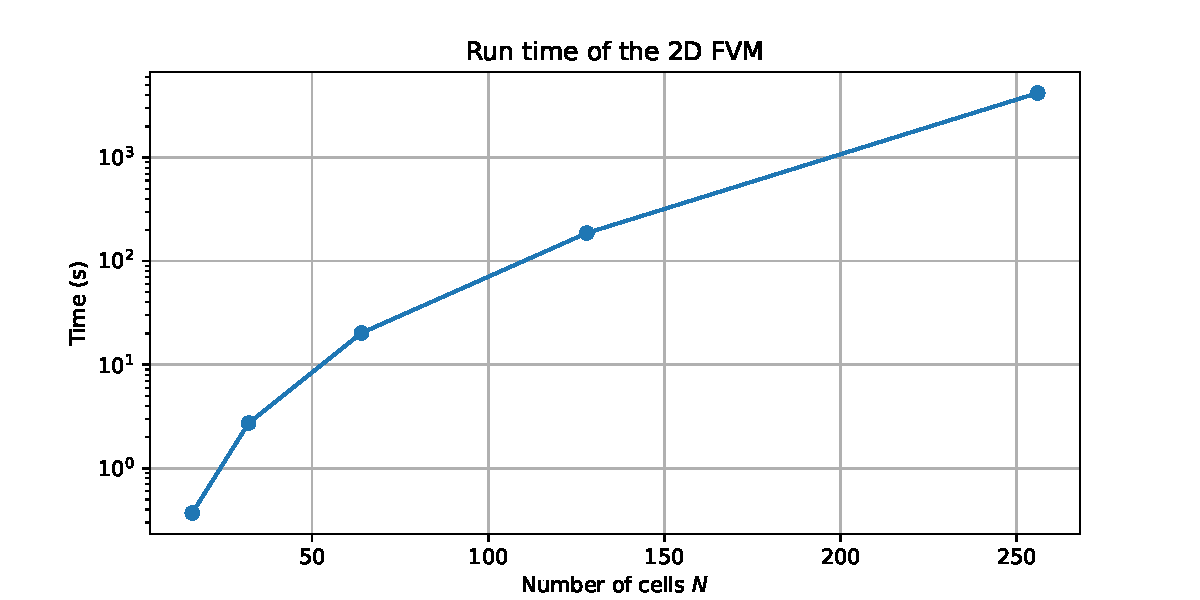
\includegraphics[width=0.8\textwidth]{C:/Users/Matteo/Shallow-Water-Equations/plots/scalability_FVM_2D.pdf}
    \caption{Scalability of the FVM to solve the 2D SWE.}\label{fig:scalability_FVM_2D}
\end{figure}
From \autoref{tab:scalability} and \autoref{fig:scalability_FVM_2D} we see that the run time increases drastically with the number of cells $N$.
This is expected, as the number of cells increases, the number of computations increases as well.
This also means that the computational cost increases with the number of cells, and the method is not scalable for large values of $N$.
Ultimately, if we want to model floods or tsunamis for the real world, we need a scalable method.
This is also some of the motivation for using data-driven methods, as we will investigate if they can be more scalable.

\section{Animations}
To visualise the results from the numerical experiments, we have created animations for the 2D idealised circular dam break problem and the SWE with a Gaussian initial condition on a sphere.
The QR-code in \autoref{fig:2D_dam_break_qr} can be used to access the animation for the 2D idealised circular dam break problem for $t=0$ s to $t = 10$ s.
\begin{figure}[H]
    \centering
    
\includegraphics[width=0.3\textwidth]{C:/Users/Matteo/Shallow-Water-Equations/QR/toro2D_dambreak_FVM_17012025_N=64_t=10_qr.png}
    \caption{QR-code for the 2D idealised circular dam break problem.
            All animations can be found at: \url{https://github.com/MelissaJessen/Shallow-Water-Equations-Animations/blob/main/README.md}.}\label{fig:2D_dam_break_qr}
\end{figure}
In the animation we observe what happens after the time steps in \autoref{fig:2D_dam_break_grid}.
We note that when the waves hit the boundaries, they are reflected back into the domain, demonstrating the behaviour of the boundary conditions.
We have also created an animation for the SWE with a Gaussian initial condition on a sphere, which can be accessed through the QR-code in \autoref{fig:2D_dam_break_qr_part2}.
\begin{figure}[H]
    \centering
    
\includegraphics[width=0.3\textwidth]{C:/Users/Matteo/Shallow-Water-Equations/QR/sphere_gaussian_FVM_17012025_qr.png}
    \caption{QR-code for the SWE with initial Gaussian conditions, projected on a sphere.
            All animations can be found at: \url{https://github.com/MelissaJessen/Shallow-Water-Equations-Animations/blob/main/README.md}.}\label{fig:2D_dam_break_qr_part2}
\end{figure}
Note, that since the SWE is solved in a 2D cartesian domain and wrapped to a sphere, we observe non-physical behaviour, especially close to the poles.


